\documentclass{beamer}
\usetheme{Warsaw}

\usepackage[utf8]{inputenc}
\usepackage{fancybox}
\usepackage{multimedia} 
\usepackage{subfig}
\usepackage{amsmath}
\usepackage{hyperref}
\hypersetup{
    colorlinks=true,     
    urlcolor=blue
}
\usepackage[all]{xy}
\begin{document}


\title[Stochastik] % (optional, only for long titles)
{Stochastik für Informatiker
\\
\includegraphics[scale=0.5]{img/craps}
}
\subtitle{}
\author[Dr. Johannes Riesterer] % (optional, for multiple authors)
{Dr.  rer. nat. Johannes Riesterer}

\date[KPT 2004] % (optional)
{}

\subject{Stochastik}


\frame{\titlepage}
\begin{frame}
    \frametitle{Informationstheorie}
\framesubtitle{}
\begin{block}{Motivation}
Die Informationstheorie ist eine mathematische Theorie aus dem Bereich der Wahrscheinlichkeitstheorie und Statistik, die auf den US-amerikanischen Mathematiker Claude Shannon zurückgeht. Sie beschäftigt sich mit Begriffen wie Information und Entropie, der Informationsübertragung, Datenkompression und Kodierung sowie verwandten Themen. 
\end{block}


\begin{block}{Motivation}
Vor allem Claude Shannon lieferte in den 1940er bis 1950er Jahren wesentliche Beiträge zur Theorie der Datenübertragung und der Wahrscheinlichkeitstheorie.

Er fragte sich, wie man eine verlustfreie Datenübertragung über elektronische Kanäle sicherstellen kann. Dabei geht es insbesondere darum, die Datensignale vom Hintergrundrauschen zu trennen. 
\end{block}

 \end{frame}




\begin{frame}
    \frametitle{Informationstheorie}
\framesubtitle{}
\begin{block}{Setting}
Gegeben eine reelle, diskrete Zufallsvariable $X :\mathcal{X} \to \mathbb{R}$ mit endlichem Grundraum $\#\mathcal{X}  \geq 2$ und Verteilung $Q$.
\end{block}

\begin{block}{Setting}
Angenommen, wir könnten Ja-Nein-Fragen stellen, um den Wert von $X$ zu bestimmen, nachdem das Zufallsexperiment ausgegangen ist.

\end{block}

 \end{frame}


\begin{frame}
    \frametitle{Informationstheorie}
\framesubtitle{}
\begin{block}{Setting}
Mit $L : \mathcal{X} \to \mathbb{N}$ bezeichnen wir die Anzahl an Fragen $L(x)$, die benötigt werden, um bei einer gewählten Strategie den Wert von $X = x$ zu erraten.
\end{block}

\begin{block}{Mittlere Anzahl an Fragen}
Wir suchen eine Strategie, so dass die mittlere Anzahl an Fragen  (Erwartungswert) $EL(X) := \sum_{x \in \mathcal{X}} L(x) Q(x)$  möglichst klein ist.
\end{block}

 \end{frame}


\begin{frame}
    \frametitle{Informationstheorie}
\framesubtitle{}

\begin{block}{Beispiel}
 $\mathcal{X} = \{ 1,2,3,4,5,6 \}$ und $Q$ die Gleichverteilung auf $\mathcal{X}$.
\end{block}

\begin{block}{Strategie 1}
$X = 1$, $j: X = 1, n: X = 2$; $j: X = 2, n:X= 3$; $j:X = 3, n:X= 4$; $j:X = 4, n:X= 5$; $j:X = 5, n:X= 6$ 
Hier ist $L(x) = \min(x,6)$ und $EL(X) = \frac{10}{3}$.
\end{block}

 \end{frame}

\begin{frame}
    \frametitle{Informationstheorie}
\framesubtitle{}
\begin{figure}[htp]
      \centering
    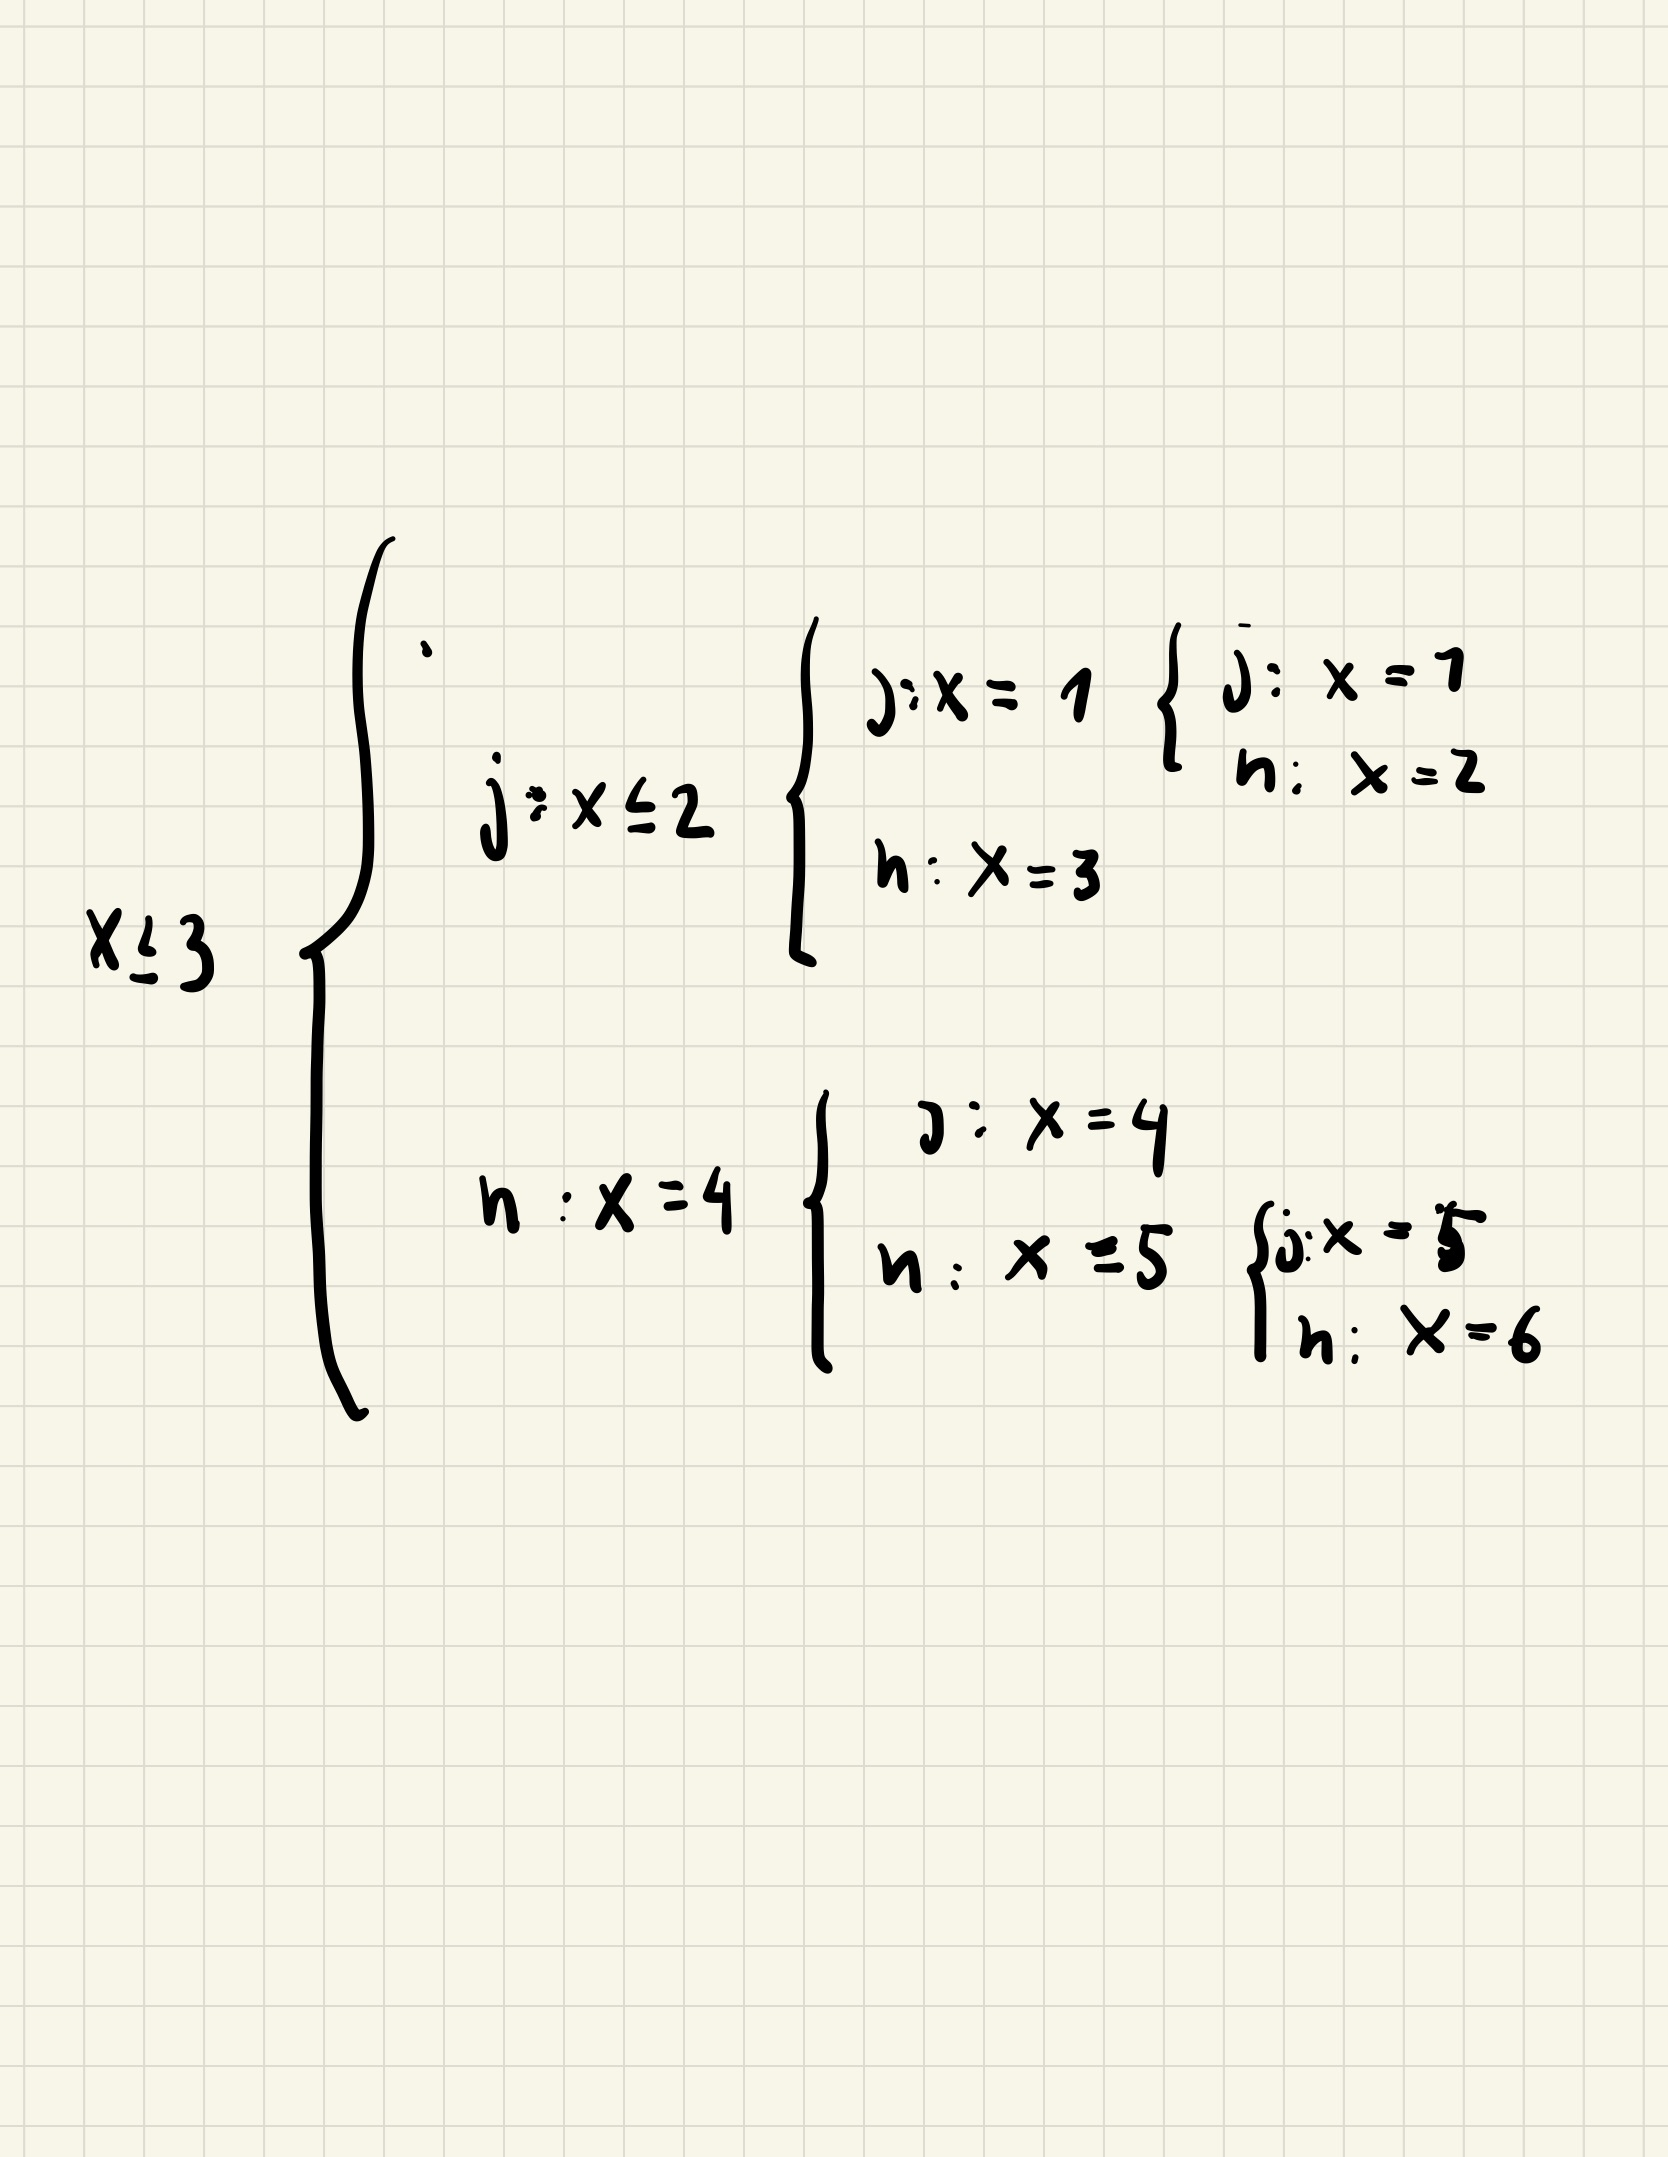
\includegraphics[width=0.45\textwidth]{img/strategie2}
\end{figure}

\begin{block}{Strategie 1}
 $EL(X) = \frac{8}{3}$.
\end{block}

 \end{frame}

\begin{frame}
    \frametitle{Informationstheorie}
\framesubtitle{}

\begin{block}{Wörter}
Gegeben sei eine endliche Menge $\mathcal{A}$ mit $\# A \geq 2$, genannt Alphabet.
Ein Wort der Länge $k$ ist gegeben durch ein Tupel $w = b_1b_2 \cdots b_k$ mit Buchstaben $b_k \in \mathcal {A}$.
\end{block}

\begin{block}{Wortmenge}
Die Menge aller Wörter bezeichnen wir mit 
$$\mathcal{W} (\mathcal{A}) := \{  b_1 \cdots b_k \; | \; k \in \mathbb{N}, \; b_i \in \mathcal{A} \} $$
 Mit $l(w):= k$ für $w=b_1 \cdots b_k  $ bezeichnen wir die Länge des Wortes.
\end{block}

 \end{frame}


\begin{frame}
    \frametitle{Informationstheorie}
\framesubtitle{}

\begin{block}{Kode}
Ein $\mathcal{A}$-Kode für die Menge $\mathcal{X}$ mit Alphabet $\mathcal{A}$ ist eine injektive Abbildung (1-zu-1)
$$ \kappa : \mathcal{X} \to \mathcal{W} (\mathcal{A})$$
die jedem Wort $x \in \mathcal{X}$ eindeutig ein Kodewort $\kappa(x)$ zuordnet.
\end{block}


\begin{block}{Präfixfreier Kode}
Ein Wort $v = a_1 \cdots a_j$ heisst Präfix des Wortes $w = b_1 \cdots b_k$, wenn $j \leq k$ und $v = b_1 \cdots b_j$ ist. Das Wort $w$ heisst Fortsetzung von $v$. Ein Kode $$ \kappa : \mathcal{X} \to \mathcal{W} (\mathcal{A})$$
 heisst präfixfrei, wenn kein Codewort $\kappa(x)$ Präfix eines anderen Kodewortes $\kappa(y)$ ist. 
\end{block}

 \end{frame}


\begin{frame}
    \frametitle{Informationstheorie}
\framesubtitle{}

\begin{block}{Präfixfreier Kode}
Für einen präfixfreien Kode gilt 
$$ \kappa(x_1 \cdots x_m) = \kappa(x_1) \cdots \kappa(x_m)$$
\end{block}

\begin{block}{Beispiel}
Sei $\mathcal{X}$ die Menge aller Telefonanschlüsse. Dann entsprechen Telefonnummern einem präfixfreien Kode über dem Alphabet $\mathcal{A} := \{0, 1,2,3,4,5,6,7,8,9\}$
\end{block}

\begin{block}{Beispiel}
$A \rightarrow 0, B  \rightarrow 100, C \rightarrow 101, D \rightarrow 11$ 
\end{block}

 \end{frame}


\begin{frame}
    \frametitle{Informationstheorie}
\framesubtitle{}

\begin{block}{Kodebaum}
Die Knotenmenge besteht aus dem Wurzelknotem und Wörtern, die Präfix eines Kosewortes sind. Die Kantenmenge besteht aus Paaren von direkten Nachfolgern.
\end{block}
\begin{figure}[htp]
      \centering
    \includegraphics[width=0.65\textwidth]{img/Kodebaum}
\end{figure}
 \end{frame}



\begin{frame}
    \frametitle{Informationstheorie}
\framesubtitle{}

\begin{block}{Zusammenhang mit Fragestrategie}
Jede Fragestrategie liefert einen präfixfreien Kode mit Alphabet $\mathcal{A := \{  \text{j} ,\text{n} \}}$.
\end{block}

\begin{block}{Zusammenhang mit Fragestrategie}
Maß für Informationsgehalt der Quelle $X$ ist nun also das Minimum von $El(\kappa (X))$ über alle präfixfreien Kodes $\kappa$ für $X$.
\end{block}

\begin{block}{Zusammenhang mit Fragestrategie}
Wir beschäftigen uns nun mit der Frage ob  man diese Größe abschätzen kann.
\end{block}


 \end{frame}



\begin{frame}
    \frametitle{Informationstheorie}
\framesubtitle{}

\begin{block}{Kraftsche Ungleichung a)}
Sei $\kappa$ ein präfixfreier $\mathcal{A}$-Kode für $\mathcal{X}$ mit $\# \mathcal{A} = d$. Dann ist
$$ \sum_{x \in \mathcal{X} }  d^{-l( \kappa(x))} \leq 1$$
\end{block}

\begin{block}{Kraftsche Ungleichung b)}
Für $x \in \mathcal{X}$ sei $L : \mathcal{X} \to \mathbb{N}$ eine Abbildung, so dass $ \sum_{x \in \mathcal{X} }  d^{-L(x)} \leq 1$ gilt. Dann gibt es einen präfixfreien  $\mathcal{A}$-Kode für $\mathcal{X}$ mit 
$$ l(\kappa(x)) = L(x) \; .$$
\end{block}


 \end{frame}

\begin{frame}
    \frametitle{Informationstheorie}
\framesubtitle{}

\begin{block}{Beweis a)}
Nehmen wir an, wir wählen zufällig ein Kodewort aus.
In jedem Knoten gibt es maximal $d$ Kanten. Damit ist $P(\kappa(x)) \geq d^{-l(\kappa(x))}$ und somit
$$ 1 = \sum_{x \in \mathcal{X}} P(\kappa(x)) \geq  \sum_{x \in \mathcal{X}} d^{-l(\kappa(x))} \; .$$
\end{block}

\begin{block}{Beweis b)}
Für $k \in \mathbb{N}$ sei $\mathcal{X}_k := \{ x \in \mathcal{X} \;  |  \; L(x) = k\}$  und $n_k := \# \mathcal{X}_k$.
Damit ist 
$$  \sum_{x \in \mathcal{X} }  d^{-L(x)} =   \sum_{k \in \mathbb{N}}  n_k d^{-k} \leq 1\;(*) .$$
Wir wählen nun induktiv Kodewörter für alle $x_k \in \mathcal{X}_k$. 
\end{block}

 \end{frame}


\begin{frame}
    \frametitle{Informationstheorie}
\framesubtitle{}

\begin{block}{ Induktions Anfang}
Nach $(*)$ ist $n_1d^{-1} \leq 1$. Daher können wir jedem $x \in \mathcal{X}_1$ einen einzelnen Buchstabe $\kappa(x) \in \mathcal{A}$ zuordnen.
\end{block}

\begin{block}{ Induktions Schritt}
Haben für alle $x \in \mathcal{X}_1 \cup \cdots \cup \mathcal{X}_m$ ein Wort $\kappa(x)$ gewählt, so dass kein Wort präfix eines  anderen ist. Jedes bereits gewählte Kodewort $\kappa(x)$ hat $d^{m+1 - l(\kappa(x))}$ Fortsetzungen zu einem Wort in $\mathcal{X}_k$. Diese stehen nicht zur Verfügung, da man sonst keine präfixfreie Kodierung erhält. Es bleiben also noch 
$$ d^{m+1} - \sum_{x \in \mathcal{X}_1 \cup \cdots \cup \mathcal{X}_m } d^{m+ 1 - L(x)} = d^{m+1} - \sum_{k=1}^{m} n_k d^{m+1-k}$$ 
Wörter übrig, die für die präfixfreie Kodierung verwendet werden können.
\end{block}

 \end{frame}


\begin{frame}
    \frametitle{Informationstheorie}
\framesubtitle{}



\begin{block}{ Induktions Schritt}
Mit $(*)$ folgt
\begin{align*}
& d^{m+1} - \sum_{k=1}^{n} n_k d^{m+1-k} = d^{m+1} (1 - \sum_{k=1}^{m} n_k d^{-k}) \\
& \geq d^{m+1}(n_{m+1} d^{-(m+1)}) = n_{m+1}
\end{align*}
Es gibt also noch genügend Wörter, um alle Punkte $x_{m+1}$ präfixfrei zu kodieren.
\end{block}

 \end{frame}


\begin{frame}
    \frametitle{Informationstheorie}
\framesubtitle{}

\begin{block}{Entropie}
Die Entropie $H_d(X)$ der Ordnung $d$ der Zufallsvariable $X$ ist definiert als das Minimum von $\sum_{x \in \mathcal{X} }  L(x) Q(x)$ über alle Abbildungen $L: \mathcal{X} \to \mathbb{N}$ mit $\sum_{x \in \mathcal{X} }  d^{-L(x)} \leq 1$.
\end{block}

\begin{block}{Entropie}
Die Entropie der Zufallsvariable $X$ ist definiert durch 
$$ H(X) := -\sum_{x \in \mathcal{X} }   Q(x) \log(Q(x))$$
\end{block}


 \end{frame}

\begin{frame}
    \frametitle{Informationstheorie}
\framesubtitle{}

\begin{block}{Entropie-Ungleichung}
Es gilt
$$ \frac{H(X)}{\log(d)} \leq H_d(X) \leq \frac{H(X)}{\log(d)} +1 \; .$$
\end{block}

 \end{frame}

\begin{frame}
    \frametitle{Informationstheorie}
\framesubtitle{}

\begin{block}{Beweis}
Die untere Abschätzung erhalten wir, indem wir  anstatt der Menge Abbildungen $L: \mathcal{X} \to \mathbb{N}$ die Menge $D$ aller 
Abbildungen $L: \mathcal{X} \to [0, \infty)$ betrachten. Für eine solche Abbildung definieren wir $f(L): = \sum_{x \in \mathcal{X}} Q(x) L(x)$ und 
$g(L):= \sum_{x \in \mathcal{X}} d^{-L(x)}$. Gesucht wir nun also das Minimum
$$ \min_{L \in D : g(L) \leq 1} f(L)$$

\end{block}

 \end{frame}


\begin{frame}
    \frametitle{Informationstheorie}
\framesubtitle{}

\begin{block}{Lagrange Multiplikatoren}
Seien $f$ und $\varphi = (\varphi_1, \cdots , \varphi_k)$ stetig differenzierbar auf einer offenen Menge $U \subset \mathbb{R}^n$ und
 $M := \{  x \in U | \varphi(x) = 0 \}$.
Die Matrix $d \varphi(x)$ habe in jedem Punkt $x \in M$ den Rank $k$. Ist $x_0 \in M$ ein Extremum von $f$ auf $M$, dann gibt es Zahlen $\lambda_1, \cdots , \lambda_n \in \mathbb{R}$ mit
$$ f'(x_0) = \sum_{i= 1}^k \lambda_i \varphi'_i(x_0) \; .$$ 
\end{block}

 \end{frame}



\begin{frame}
    \frametitle{Informationstheorie}
\framesubtitle{}

\begin{block}{Beweis}
Sei $x_0$ ein Extremum von $f$ in $M$ und $\gamma$ eine Kurve mit $\gamma(0)= x_0$ und $\gamma'(0) = v$.
Die Funktion $F(t) := f(\gamma(t))$ hat in $t= 0$ ein Extremum und damit $F'(0) = 0$ und mit der Kettenregel $<\nabla f(x_0), v> = 0$.
Die Funktionen $\varphi_i'(x_0)$ erfüllen ebenfalls $<\varphi_i' (x_0),v> = 0$ und da der Rang von $d \varphi(x)= k$ ist, bilden  $\varphi_1, \cdots , \varphi_k$ eine Basis des Vektorraums der Vektoren, die senkrecht auf $M$ stehen.
\end{block}

 \end{frame}



\begin{frame}
    \frametitle{Informationstheorie}
\framesubtitle{}

\begin{block}{Beweis Entropie-Ungleichung weiter }
Wollen Minimum finden  
$$ \min_{L \in D} \sum_{x \in \mathcal{X}} Q(x) L(x) + \lambda d^{-L(x)}$$
für ein $\lambda > 0$. Summandenweise ist
$$\frac{d}{dr} Q(x) r + \lambda d^{-r} =  Q(x) - \lambda \log(d) e^{-\log(d)r}$$
Somit ist  $L_0(x) := \frac{\frac{- \log Q(x)}{\lambda \log(d)}}{\log(d)}$ eine Nullstelle und damit ein Minimum. Mit $\lambda = \frac{1}{\log(d)}$ ist $L_0(x) = -\log_d Q(x)$  und damit $g(L_0) = 1$. Somit ist
$$ H_d(X) \geq f(L_0) = - \sum_{x \in \mathcal{X}} \log_d (Q(X)) = \frac{H(X)}{\log(d)}$$ 

 \end{block}

 \end{frame}


\begin{frame}
    \frametitle{Informationstheorie}
\framesubtitle{}

\begin{block}{}
Definieren wir $L(x) = \lceil L_0(x) \rceil$. Dann ist 
$$ \sum_{x \in \mathcal{X}} d^{-L(x)} \leq \sum_{x \in \mathcal{X}} d^{-L_0(x)} \leq = 1$$
und mit $0 \leq L - L_0 < 1$ 
$$ H_d(X) \leq  \sum_{x \in \mathcal{X}} Q(x) L(x) <  \sum_{x \in \mathcal{X}} Q(x) (L_0(x) +1) = \frac{H(Q)}{\log(d)} +1$$ 
\end{block}

 \end{frame}

\begin{frame}
    \frametitle{Informationstheorie}
\framesubtitle{}

\begin{block}{Konstruktion fast optimaler Kodes}
Berechne für $x \in \mathcal{X}$ die Funktion $L(x) := \lceil -\log_d(Q(x)) \rceil$. Damit erhält man einen präfixfreien $\mathcal{A}$-Kode
$\kappa$ mit $l(\kappa(x)) = L(x)$. Wie eben gezeigt gilt dann $El(\kappa(X)) < H_d(Q) +1$.
\end{block}

 \end{frame}


\end{document}
